\documentclass[11pt]{article}

% ============================================================================
%  Token-Safer (English). Build: tectonic vs-token-safer.tex
%  Figures: figures/*.pdf  (regenerate from SVG with: python figures/build.py)
% ============================================================================

\usepackage[utf8]{inputenc}
\usepackage[T1]{fontenc}
\usepackage{lmodern}
\usepackage{microtype}
\usepackage[margin=1in]{geometry}
\usepackage{amsmath,amssymb}
\usepackage{booktabs}
\usepackage{graphicx}
\usepackage{xcolor}
\usepackage{hyperref}
\usepackage{url}
\hypersetup{colorlinks=true, linkcolor=blue!55!black, citecolor=blue!55!black, urlcolor=blue!55!black}

\setlength{\emergencystretch}{3em}
\sloppy

\title{\textbf{Token-Safer: Enforcing Official Language-Server Indices over
Grep for Zero-Transmission, Token-Capped Code Search in LLM Coding Agents}}

\author{
  Sungmin Jeon\\
  \texttt{sungmin1505104@gmail.com}
}
\date{June 2026}

\begin{document}
\maketitle

\begin{abstract}
Coding agents read repositories through tool calls, and every result competes for
the same context window the model reasons in. The usual tool is \texttt{grep}, and
its output is pasted in whole.

This is cheap to run but wasteful to read. A text scan cannot separate a function
from a same-named variable or a comment, so it returns matches the model must read
and discard. Its cost also grows with the match count, not with the answer.

We present \textbf{vs-token-safer} (\texttt{vts}), a local-only Model Context
Protocol (MCP) server and CLI. It routes each search to an \emph{official} language
server --- clangd, a Roslyn server, \texttt{typescript-language-server}, pyright ---
instead of building its own index. It caps every answer to a compact
\texttt{file:line} list, with no source bodies. And it makes the substitution stick
by rewriting \texttt{grep} into the equivalent capped call at the hook layer.

Nothing is stored, embedded, or sent over the network. Across a 74-check harness
and several months of single-developer use, capped output is about $2\times$
smaller than the raw index response, and up to $10.7\times$ smaller on the heaviest
query. The hook absorbs hundreds of thousands of \texttt{grep} tokens per month on
a large game-engine tree. For navigation, references, and renames, \texttt{vts} is
a safer and cheaper substitute for \texttt{grep}. We also state where \texttt{grep}
remains the better tool.
\end{abstract}

\section{Introduction}
\label{sec:intro}

When an agent opens an unfamiliar repository, it searches first. Three questions
dominate: where is \texttt{X} defined, what calls \texttt{Y}, and where is
\texttt{Z} used. In almost every agent today, all three are answered by
\texttt{grep} or \texttt{ripgrep}, and the result is placed verbatim into the
model's context.

This is convenient, but it carries two costs. The first is precision. A text scan
matches every occurrence, including hits in comments and string literals, unrelated
identifiers that share a substring, and overloads the agent did not ask about. The
model spends tokens reading these and attention discarding them.

The second cost is volume. The token count of a grep result scales with the number
of matching lines and the surrounding context, not with the size of the answer.
For a ``where is it'' question, that answer is only a short list of positions.

Language servers already solve the precision half. The Language Server Protocol
(LSP) exposes semantic operations --- definition, references, document and
workspace symbols, call hierarchy, and rename --- over a real parser and type
resolver. A reference query therefore returns the actual referents, not textual
look-alikes. Reported results agree: for renames, type checks, and call-chain work,
an LSP is the right backend, and a lookup that costs roughly two thousand grep
tokens can be answered in about five hundred LSP
tokens~\cite{lsp-medium,semble-hn}. Anthropic added native LSP support to Claude
Code in late 2025~\cite{anthropic-lsp}.

Two questions remain open. How should an agent be \emph{made} to use that index
rather than merely offered it? And what should be allowed to cross from the index
into the model's context? \texttt{vts} takes a definite position on both, stated as
three commitments.

\begin{enumerate}
  \item \textbf{Reuse the official engine; ship only the glue.} Indexing C++, C\#,
  TypeScript, and Python correctly is hard, and clangd, Roslyn, \texttt{tsserver},
  and pyright already do it. A token saver should be a thin LSP-to-MCP adapter ---
  not a re-implemented parser, and not a third-party index over someone's source.

  \item \textbf{Cap the answer, not just the question.} The saving comes as much
  from refusing to return bodies as from asking a semantic question. Every answer
  is a de-duplicated, directory-factored \texttt{file:line} list, so less source
  reaches the model than under grep-and-paste. The privacy story and the token
  story improve together.

  \item \textbf{Enforce the swap; do not merely offer it.} An agent that
  \emph{could} call a better tool still reaches for \texttt{grep} by habit. We
  rewrite a single safe \texttt{grep} call into the matching capped call at the
  pre-tool hook, leaving the agent's flow intact while removing the bypass.
\end{enumerate}

\paragraph{Contributions.}
This paper contributes: (i) a thin LSP-to-MCP adapter that fronts four official
language servers behind one capped, per-call-rooted tool surface
(Section~\ref{sec:arch}); (ii) an output-compaction scheme --- positions only,
file-grouped, prefix-factored --- measured at about $2\times$ over raw index
responses and up to $10.7\times$ on the heaviest query (Sections~\ref{sec:cap}
and~\ref{sec:eval}); (iii) a hook layer that rewrites grep into the equivalent
capped call and that quantifies, then steers, both the grep habit and a second
whole-declaration edit habit (Section~\ref{sec:enforce}); and (iv) a reproducible
74-check harness with live verification against clangd, Roslyn, \texttt{tsserver},
and pyright on real projects (Section~\ref{sec:eval}).

\paragraph{A contrasting design.}
\emph{Codebase-Memory}~\cite{cbm} attacks the same token problem from the opposite
direction. It builds a \emph{persistent} Tree-Sitter knowledge graph over 66
languages, with optional embedded vector search and a local visualization.
\texttt{vts} inverts each of those choices: on-demand official-LSP queries instead
of a stored graph, compiler-grade engines instead of a hand-written parser, and a
hard no-transmission rule instead of embeddings. That contrast organizes the rest
of the paper (Section~\ref{sec:related}).

\section{Background and Related Work}
\label{sec:related}

\paragraph{Grep as the search backbone.}
Lexical search is the default for sound reasons. It needs no build, it ignores file
type, and it searches everything --- which is what an agent wants in its first
minutes inside an unknown tree~\cite{yage-grep}.

Its weaknesses are equally clear. It cannot separate a symbol from a substring, and
nothing bounds its output to the relevant~\cite{lsp-medium}. Newer agent-search
tools such as Semble report up to a $98\%$ token reduction against grep by returning
structured, de-duplicated results~\cite{semble-hn}. We take the lesson that grep
should be bounded and complemented, not forwarded blindly.

\paragraph{LSP for agents.}
A growing body of work wires LSP into coding agents to provide semantic navigation
and live diagnostics in place of text
matching~\cite{lsp-medium,anthropic-lsp,hyperagent}. \texttt{vts} belongs to that
family but shifts the emphasis. It is not only an LSP client but an LSP enforcer
with a hard output cap, and it ships as a drop-in MCP plugin plus a hook that
substitutes for grep, rather than as a set of optional tools.

\paragraph{Why we did not build our own index.}
The obvious alternative is to build a semantic index, as
Codebase-Memory~\cite{cbm} does. It stores a Tree-Sitter knowledge graph with its
own type resolver and optional embeddings, and reports good token savings across 31
repositories. It is a capable design. We chose the opposite, for three reasons.

First, a stored graph is a second copy of the truth. It drifts from the source and
must be invalidated and rebuilt.

Second, a hand-written parser is a second implementation. It can disagree with the
compiler the project actually uses, and then the agent receives answers the build
would not.

Third, embeddings add a place for data to be stored and sent, which breaks the
zero-transmission rule we want to keep.

\texttt{vts} therefore stores no semantic database, hands every semantic question
to the build's own compiler front end, and transmits nothing. We do borrow two
ideas from that work --- an on-demand call graph and content-hash invalidation ---
but we build them as ephemeral LSP queries and a small local cache, not a stored
graph (Section~\ref{sec:beyond}).

\section{Design Principles}
\label{sec:principles}

Four invariants govern \texttt{vts}, and each is checked by the regression harness
(Section~\ref{sec:eval}).

\begin{description}
  \item[P1 --- Official engine, our glue.] clangd (LLVM) and the Roslyn-based
  server (Microsoft) perform the analysis; we write the LSP-to-MCP adapter and
  nothing more. We never reuse a third-party MCP server over source, and never
  re-implement a parser.

  \item[P2 --- Token-first.] Every feature must hold or improve the token win.
  Output is \texttt{file:line}, capped, with no bodies, and a new feature ships only
  with a harness check that asserts its output stays capped.

  \item[P3 --- Local-only, zero-transmission.] There are no network calls; nothing
  is embedded, uploaded, or reported. Because the cap returns positions rather than
  bodies, less source crosses into the model than under grep-and-paste. The privacy
  argument and the token argument coincide.

  \item[P4 --- Enforced, not optional.] A better tool the agent forgets to call
  saves nothing. The swap is enforced at the hook by rewriting a grep call into the
  matching capped call, with graceful fallbacks when rewriting is unsafe.
\end{description}

\section{System Architecture}
\label{sec:arch}

\texttt{vts} presents three faces over one core. An MCP server exposes a small,
fixed tool set to the agent: thirteen first-class tools, plus a single
\texttt{vts\_admin} tool that folds nine rarely-used administrative operations so
they do not clutter the surface. A \texttt{vts} CLI exposes the same operations to a
shell. A set of hooks intercepts and rewrites grep-class calls.

Figure~\ref{fig:layers} shows how the pieces stack, and Figure~\ref{fig:arch}
traces a single request through them.

\begin{figure}[h]
\centering
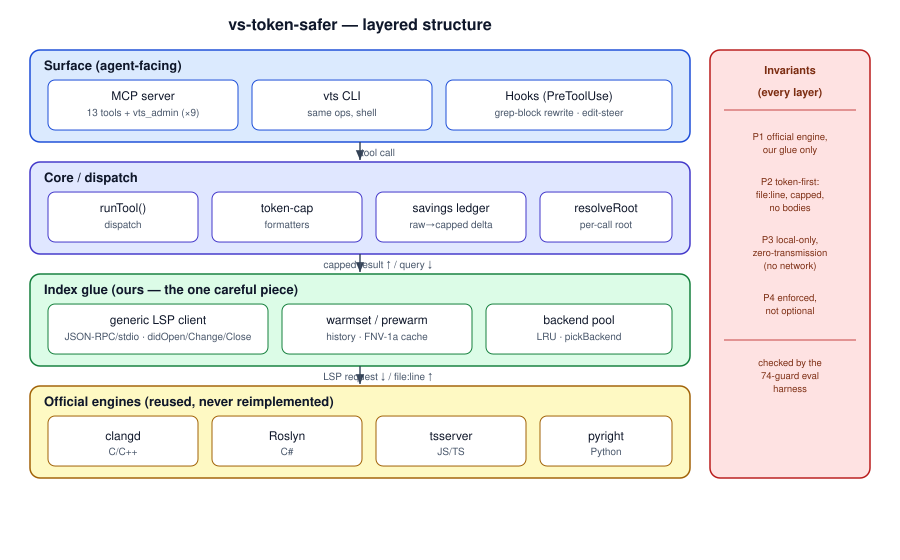
\includegraphics[width=0.96\linewidth]{figures/layers.pdf}
\caption{The four layers, from the agent-facing surface down to the official
engines, with the four invariants (P1--P4) that every layer must honor and that the
eval harness checks. We author only the index-glue layer; the engines are reused
as-is.}
\label{fig:layers}
\end{figure}

\begin{figure}[h]
\centering
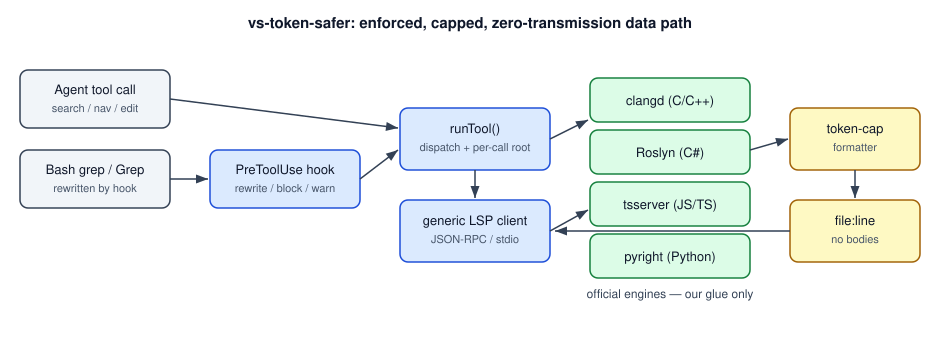
\includegraphics[width=\linewidth]{figures/architecture.pdf}
\caption{The request path. Agent tool calls and rewritten grep commands enter a
single \texttt{runTool} dispatch, which drives a generic LSP client over the
official language server for the target file. The formatter caps the reply to a
\texttt{file:line} list before it reaches the model. Nothing leaves the host.}
\label{fig:arch}
\end{figure}

\subsection{Generic LSP client}
The one genuinely new and delicate part is a generic JSON-RPC-over-stdio LSP
client. Two behaviors matter.

The first is open-or-refresh document sync. The first reference to a file sends
\texttt{didOpen} at version~1. A second reference to an already-open file sends
\texttt{didChange} with a bumped version and the file's current disk text, so an
edit made after warm-up is never answered from a stale buffer. A deleted file sends
\texttt{didClose}. Position-based tools re-open before each query, so hover, goto,
outline, and rename always read the file as it is now.

The second is spec-conformant replies to the server. The server also makes requests
of the client, and those receive shape-correct answers: an array for
\texttt{workspace/configuration}, \texttt{\{applied:false\}} for
\texttt{workspace/applyEdit}, and so on. A timed-out request is followed by
\texttt{\$/cancelRequest}, and an unknown method returns \texttt{MethodNotFound}.
These details are minor, but they keep a real language server from stalling.

\subsection{Backend selection for mixed repositories}
A repository often holds more than one language, so the backend is chosen per
query. Detection prefers the strongest build artifact, in the order
\texttt{compile\_commands.json} $\rightarrow$ clangd,
\texttt{.sln}/\texttt{.csproj} $\rightarrow$ Roslyn,
\texttt{tsconfig}/\texttt{package.json} $\rightarrow$ TypeScript, and
\texttt{pyproject}/\texttt{*.py} $\rightarrow$ pyright.

A query that names a specific file overrides that order and routes by the file's own
extension first. This single rule prevents a \texttt{.py} or \texttt{.ts} file
inside a C++-rooted tree from being handed to clangd, which would find nothing and
teach the agent to abandon the tool.

A single globally installed server resolves the correct project root per call by
walking up to the nearest project marker, and it bounds resident memory with an LRU
pool of warm backends (default cap two, idle clients reaped after five minutes).

\subsection{Warm set and prewarming}
Because language servers index asynchronously, cold latency dominates the first
query. \texttt{vts} steers the server's open set toward what is likely to be asked.

Prewarm candidates are ordered by prior query history, then currently-edited files
(from \texttt{git status} or Perforce \texttt{opened}), then recent git-log files,
then include-graph centrality, then modification time.

The include-graph cache is keyed on a composite of modification time, size, and an
FNV-1a content hash. It therefore reuses a cached result when the bytes are
unchanged despite timestamp jitter, yet still notices a real edit that a
timestamp-only key would miss. Per-language warm caps scale to each language's file
count, so a mixed-language repository warms in proportion to its makeup.

\section{Token-Capping and Output Compaction}
\label{sec:cap}

The token win is produced by the formatters, not merely by the choice of a semantic
query. Three strategies do the work.

\emph{Positions, not bodies.} Answers are \texttt{file:line}. A body is read only
when the agent explicitly asks for one, and even editing is offered by symbol name
(Section~\ref{sec:beyond}).

\emph{Repetition collapse.} A references-heavy answer is grouped by file --- one row
per file, with its line numbers joined, de-duplicated, and sorted, as in
\texttt{Foo.cpp:42,88,120}. The shared directory prefix is then factored out once.
Every location survives and is recoverable as prefix plus tail. On a deep reference
result this compounds from roughly $4\times$ for the coalescing to roughly
$10\times$ once the prefix is removed.

\emph{Outline noise suppression.} Document outlines hide anonymous callbacks and
nested local variables by default, keeping the declaration structure and a count of
what was hidden. In one case a 105-symbol file outline dropped to 32 visible
entries.

\emph{Ranking before the cap.} Because the cap keeps only the top-N rows, their
order decides whether the row the model wants is shown at all. We therefore rerank
the engine's own results before capping: by lexical match quality (exact, prefix,
word or camel boundary, then plain substring), a small preference for callable
kinds, and a query-history signal reused from prewarming. This adopts the
lexical-plus-semantic fusion that Semble~\cite{semble-hn} found effective, but it
ranks the official engine's results rather than embedding vectors, so it adds no
index and transmits nothing. \texttt{VTS\_RANK=0} disables it.

A confident ranking lets us go one step further. When an exact-name match appears in
a large result --- the common case of locating one known symbol --- we show it and
a few neighbors instead of the full cap, leaving the rest in the overflow note and
the recovery file (\texttt{VTS\_FOCUS=0} restores the full list). And for a
multi-word query, \texttt{search\_text} ranks lines by how many of the query's terms
they carry: a lexical approximation of conceptual search that needs no embeddings
(\texttt{VTS\_CONCEPT=0} disables it). The semantic, synonym-aware form of
conceptual search would require embeddings, so it stays out of scope by the same
rule that rejects a stored index.

When an answer is capped, \texttt{vts} writes a recovery ``tee'' file so the full
set can be retrieved without re-running the query. A savings ledger records the
raw-versus-capped token delta per tool; Section~\ref{sec:eval} reads that ledger.

\section{Behavioral Enforcement}
\label{sec:enforce}

A hook intercepts \texttt{Bash} grep-class commands --- grep, rg, ack, ag, findstr,
\texttt{git grep}, and \texttt{find -name} --- along with the built-in Grep and Glob
tools.

\paragraph{Rewrite, not block.}
A single safe grep segment is rewritten, through the pre-tool hook's input-mutation
channel, into the matching \texttt{vts} CLI call. The result is token-capped and the
agent's flow is unbroken.

The segment splitter is quote-aware. It treats a \texttt{|} inside quotes as a regex
alternation rather than a shell pipeline, so the two most common bypasses,
\texttt{grep "FooA|FooB"} and \texttt{grep "\^{}\#include"}, rewrite cleanly to a
capped text search. Only an ambiguous or unsafe command --- a genuine pipeline, an
unsafe pattern, a quote in the root path --- falls back to a hard block, and even
then it prints a ready-to-run replacement.

\paragraph{Symbol-hunt classification.}
A grep that plainly enumerates symbols is routed to the semantic symbol search. The
triggers are a bare identifier, a regex carrying a code-structural cue such as
\texttt{::} or a literal \texttt{(} or a type keyword, or a CamelCase/snake
alternation such as \texttt{MaxWalkSpeed|MaxExcessSpeed}.

Keyword alternations that carry no identifier signal, such as \texttt{TODO|FIXME} or
\texttt{GET|POST}, are left as warnings to keep false positives near zero. All
enforcement is reversible through an escape-hatch environment variable, and messages
are emitted in the operator's locale.

\paragraph{Measuring and steering the edit habit.}
Search is not the only bypass. A second one is the built-in, line-based edit that
replaces or inserts a whole declaration --- something a symbol-level edit could do
by name, without first reading the file into context.

A shared classifier, used by both the offline discovery scan and the live hook,
flags those edits. It excludes control-flow blocks that merely look like
declarations, and it attributes the prior file-read tokens a symbol edit would have
skipped.

Three layers then try to convert the habit: a focused nudge riding a search result,
a model-visible warning that carries a ready symbol-edit call, and an opt-in
one-shot block of a safe insert. An adoption ledger re-injects the current adoption
ratio as a session goal, a measure-then-re-inject loop that a static instruction
cannot provide. Section~\ref{sec:discuss} reports how stubborn this habit is.

\section{Beyond Search: Navigation, Call Hierarchy, Editing, Visualization}
\label{sec:beyond}

The same capped, zero-transmission discipline extends past reference search.

\paragraph{Navigation, folded.}
\texttt{goto\_definition} folds type definition, implementation, and declaration
behind a \texttt{kind} parameter rather than spawning new tools. Hover, document
symbols, and a compact diagnostics list (compiler and linter findings rendered as
\texttt{file:line:col severity [code]: msg}) complete the read surface.

\paragraph{Call hierarchy as a fold, not a tool.}
A multi-hop call hierarchy --- the transitive callers that form the blast radius
before an edit, or the callees --- is folded \emph{into} the reference tool through
a \texttt{direction} parameter. It is implemented over the official LSP
\texttt{callHierarchy} requests with cycle and depth guards (default depth five,
eighty nodes). This is the on-demand counterpart of a persistent call graph: real
semantic edges, no stored graph, nothing transmitted, and no new tool on the
surface.

\paragraph{Symbol-level editing.}
Replace-body, insert (before or after), and a reference-checked safe-delete each
resolve a declaration by name through the LSP outline and splice text at the
symbol's span. All are preview-by-default, and safe-delete refuses while the symbol
is still referenced unless forced. Editing by naming a symbol skips reading the
whole file and counting lines for an exact match, which is the editing counterpart
of the search cap.

\paragraph{Local, zero-transmission visualization.}
An opt-in, CLI-only dashboard renders the include graph and an on-demand call graph
in 3D through a vendored, same-origin WebGL library (no CDN). It binds to loopback
only and is never started by the MCP server. It is the visualization counterpart of
the charter: a useful view where nothing leaves the host.

\section{Evaluation}
\label{sec:eval}

We evaluate along three lines: a deterministic regression harness, live
language-server verification on real projects, and several months of
single-developer usage telemetry.

We are deliberate about the distinction. The harness is controlled and
reproducible. The telemetry is real usage, and therefore observational rather than a
controlled benchmark. We do not claim a multi-repository A/B study of answer
quality. We claim that the cap holds, that the enforcement fires, and that the
realized savings are measurable.

\subsection{Regression harness}
A mock-LSP harness (\texttt{eval/run.mjs}) exercises every tool and invariant
without a toolchain present. It asserts on token-cap behavior, backend selection,
document-sync freshness, enforcement rewrites, and each new feature.

The harness currently holds \textbf{74 checks} and passes in full. Every new code
path ships with a check; this is principle~P2 in operational form. As one concrete
data point, a cold workspace-symbol query whose raw index response is about
$57{,}308$ tokens is capped to about $1{,}434$ tokens, roughly a $40\times$
reduction.

\subsection{Live language-server verification}
Each of the four backends was verified end-to-end against the official engine, not a
mock.

\begin{itemize}
  \item \textbf{C/C++ (clangd)} on a real Unreal Engine 5.x project.
  \texttt{search\_symbol} returned a game \texttt{UCLASS} and its generated symbols
  as \texttt{file:line}. Two reproducible facts came out of it. First,
  \texttt{GenerateClangDatabase} needs \texttt{-Compiler=VisualCpp} when the targets
  build with clang-cl. Second, a vendored clangd 19.1.5 deadlocks on a full game
  translation unit in server mode, while a standalone clangd $\geq 22$ parses the
  same unit in about thirteen seconds. We therefore probe the version and use a
  persisted-index fast path that returns the moment the sought symbol's shard loads.
  That path turns a $369$-second wait for the full background index into a
  $51$-second answer once the static index is loaded, a $7\times$ cut in first-query
  latency.
  \item \textbf{C\# (Roslyn-based server)} against
  Microsoft.CodeAnalysis.LanguageServer, the Visual Studio and C\# Dev Kit engine.
  \item \textbf{JavaScript/TypeScript (\texttt{typescript-language-server})}
  verified by running \texttt{vts} on its own source.
  \item \textbf{Python (pyright)} through the same generic glue as TypeScript.
\end{itemize}

\subsection{Token savings telemetry}
Over $441$ recorded searches by a single developer, the local ledger puts the capped
output about $2\times$ smaller than forwarding the raw index responses: $263{,}540$
tokens become $133{,}289$, a saving near $130{,}000$ tokens. The heaviest single
query compacts $10.7\times$, from $21{,}056$ to $1{,}961$ tokens.

Figure~\ref{fig:savings} and Table~\ref{tab:savings} break the saving down by tool.
Document-outline suppression and text-search capping dominate.

These figures count only the compaction of the search result itself. They omit the
larger and harder-to-measure half: the file reads the agent never makes because it
received \texttt{file:line} positions and a named symbol span instead of opening
files. We surface part of that read-avoidance in the ledger by baselining
\texttt{read\_symbol} against the whole file it replaces, which mirrors how Semble
reports its savings ``combined with file reading''~\cite{semble-hn}.

\begin{figure}[h]
\centering
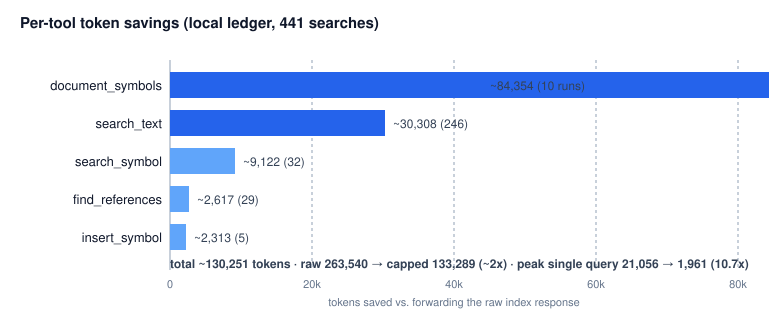
\includegraphics[width=0.92\linewidth]{figures/savings.pdf}
\caption{Per-tool token savings from the local ledger (441 searches, one developer).
These are observational usage figures, not a controlled benchmark.}
\label{fig:savings}
\end{figure}

\begin{table}[h]
\centering
\caption{Per-tool token savings from the local ledger. Observational telemetry.}
\label{tab:savings}
\begin{tabular}{lrr}
\toprule
Tool & Runs & Tokens saved \\
\midrule
\texttt{document\_symbols} & 10  & $\sim$84{,}354 \\
\texttt{search\_text}      & 246 & $\sim$30{,}308 \\
\texttt{search\_symbol}    & 32  & $\sim$9{,}122 \\
\texttt{find\_references}  & 29  & $\sim$2{,}617 \\
\texttt{insert\_symbol}    & 5   & $\sim$2{,}313 \\
\midrule
\textbf{vts total}         & 441 & $\sim$130{,}251 \\
\bottomrule
\end{tabular}
\end{table}

\subsection{Enforcement coverage}
An offline discovery scan over the agent's own session transcripts measures how much
code search bypassed \texttt{vts}. On a large game-engine workload, the matcher's
recent-window catch rate is about $68\%$.

The two enforcement upgrades aimed at symbol-hunt grep are observed to intercept
roughly $172$k tokens per month (the block on structural grep) and a further $319$k
per month (the block on CamelCase-alternation grep).

The same scan quantifies the edit habit. Over a 30-day window, $1{,}284$
whole-declaration line edits read about $468$k tokens of file content first, and
$93\%$ of them happened with no prior \texttt{vts} search on that file. That figure
measures both the opportunity and the ceiling of a search-result-only steer, and it
is why the edit-adoption ledger exists.

\subsection{Threats to validity}
We name the threats plainly.

\emph{External validity.} The savings and enforcement telemetry come from one
developer in one environment, so the absolute figures are existence proofs of the
effect, not population estimates. A different codebase mix or working style would
move them.

\emph{Construct validity.} We measure tokens saved against the raw index response,
which captures the formatting win but not whether the agent reached the same answer
it would have reached from grep. We argue correctness from the use of a semantic
engine and the live verifications, not from a task-success metric.

\emph{Internal validity.} The ledger is instrumentation inside the same process it
measures, and at least one input (the bundled log-compaction entry) is degenerate,
which is why we partition it out rather than report a combined number.

\emph{Reference quality.} Part of our related work cites practitioner posts rather
than peer-reviewed venues, reflecting how recent the agent-LSP shift is. We mark
those as such and place no load-bearing claim on them.

\subsection{Artifact availability}
\texttt{vs-token-safer} is released as an installable MCP plugin and CLI, and the
evaluation in this section is reproducible from the repository. \texttt{node
eval/run.mjs} runs the 74-check harness with no toolchain present, and \texttt{vts
savings} prints the ledger underlying Table~\ref{tab:savings}.

The figures in this paper are generated from version-controlled SVG sources
(\texttt{figures/build.py}). The numbers reported here correspond to release
v0.32.2; we recommend re-running both commands and rebuilding before citing exact
values, since the ledger advances with use.

\section{Discussion and Limitations}
\label{sec:discuss}

\paragraph{Where grep stays.}
\texttt{vts} does not abolish lexical search; it bounds it. A language server exists
only for file types that have one, while an agent's search needs cover all text in
the tree.

\texttt{vts} therefore keeps a capped text-search tool for the file-type-agnostic
case, and reserves enforcement for the cases where a semantic answer is strictly
better: symbol hunts, references, and renames. Freeform and keyword-alternation
searches are left as warnings on purpose.

\paragraph{Cold latency.}
The honest price of using a real compiler front end is first-query latency on a
cold, large index. \texttt{vts} softens it with prewarming, a persisted-index fast
path, and a poll-until-the-shard-loads strategy, but it cannot erase it. A warm IDE
that proxies an already-running language service still answers a first query sooner.
Keeping the server resident at least pays the per-spawn cost once per session rather
than once per call.

\paragraph{Adoption is behavioral, not only technical.}
The most striking measured gap is not in what the tool can do, but in whether the
agent reaches for it. With a capped symbol-edit available, the agent still defaults
to a line-based edit about nine times in ten.

A permanent hard block proved counterproductive: it traps the agent into fighting
the wall with retries. The levers that actually moved the number were a ready-to-run
suggested call and a re-injected live adoption metric. Closing this gap is the open
problem we care about most.

\paragraph{On evaluation honesty.}
Our quantitative results are usage telemetry and a deterministic harness, not a
controlled multi-repository benchmark of answer quality against grep or against a
persistent knowledge graph. The natural next step is that study: hold the agent and
the tasks fixed, vary only the search backend, and measure tokens, wall-clock, and
task success across a repository suite. We flag it as future work rather than present
the current data as more than it is.

\section{Conclusion}
\label{sec:conc}

\texttt{vs-token-safer} makes an agent's code search semantic, capped,
zero-transmission, and enforced. It reuses the official language servers as the
analysis engine and writes only the LSP-to-MCP glue. It returns positions rather
than bodies, and it rewrites grep into the matching capped call at the hook.
Together these lower the token and privacy cost of the navigation, reference, and
rename class of operations, while leaving lexical search where it belongs.

Set against a persistent knowledge graph, \texttt{vts} trades stored-index reach and
breadth of language coverage for correctness by construction --- the compiler's own
front end --- for freshness without an invalidation problem, and for a firm
no-transmission guarantee.

The problem we leave open is behavioral rather than technical: getting the agent to
reach for the cheaper tool. There, live measurement and re-injection proved more
effective than a wall.

% ============================================================================
\begin{thebibliography}{9}

\bibitem{cbm}
DeusData.
\newblock Codebase-Memory: Tree-Sitter-Based Knowledge Graphs for LLM Code
Exploration via MCP.
\newblock arXiv:2603.27277, 2026. \url{https://arxiv.org/abs/2603.27277}

\bibitem{anthropic-lsp}
Anthropic.
\newblock Native Language Server Protocol support in Claude Code (v2.0.74),
December 2025.

\bibitem{lsp-medium}
V.\ Thiagarajan.
\newblock LSP --- The Protocol Your IDE Uses Every Day (And Now Your AI Agent
Does Too). Medium, 2026.

\bibitem{semble-hn}
Semble.
\newblock Code search for agents that uses 98\% fewer tokens than grep.
Hacker News, 2026. \url{https://news.ycombinator.com/item?id=48169874}

\bibitem{yage-grep}
Yage.
\newblock Why Coding Agents Still Use grep as Their Search Backbone. 2026.
\url{https://yage.ai/share/why-coding-agents-still-use-grep-en-20260327.html}

\bibitem{hyperagent}
H.\ N.\ Phan, T.\ N.\ Nguyen, P.\ X.\ Nguyen, and N.\ D.\ Q.\ Bui.
\newblock HyperAgent: Generalist Software Engineering Agents to Solve Coding Tasks
at Scale.
\newblock arXiv:2409.16299, 2024.

\end{thebibliography}

\end{document}
